\documentclass{acm_proc_article-sp}
\usepackage{algorithmic}
\usepackage{algorithm}

\begin{document}

\title{Reward-Based Social Learning}

\numberofauthors{3}
\author{
\alignauthor
Wesley Tansey\\
       \affaddr{Dept. of Computer Science, The University of Texas at Austin}\\
       \affaddr{1 University Station C0500, Austin, TX, USA}\\
       \email{tansey@cs.utexas.edu}
\alignauthor
Eli Feasley\\
       \affaddr{Dept. of Computer Science, The University of Texas at Austin}\\
       \affaddr{1 University Station C0500, Austin, TX, USA}\\
       \email{elie@cs.utexas.edu}
\alignauthor
Risto Miikkulainen\\
       \affaddr{Dept. of Computer Science, The University of Texas at Austin}\\
       \affaddr{1 University Station C0500, Austin, TX, USA}\\
       \email{risto@cs.utexas.edu}
}
\date{25 January 2012}

\maketitle
\begin{abstract}
Social learning is an extension to evolutionary algorithms that enables agents to learn from observations of others in the population. Traditionally, social learning algorithms have employed a student-teacher model where the behavior of one or more high-fitness agents is used to train the remaining agents in the population. We present a reward-based model of social learning in which we do not label agents as teachers or students, instead allowing any individual receiving a positive reward to teach other agents to mimic its recent behavior. We validate our approach in two foraging tasks, comparing reward-based social learning with two variants of student-teacher social learning, as well as traditional neuroevolution. We show that in a complex foraging task, our reward-based approach converges to a strategy superior to that of other methods. Moreover, our algorithm discovers near-optimal solutions in both foraging tasks with up to two orders of magnitude fewer agent evaluations than any of our benchmark strategies. Our results suggest reward-based social learning can substantially speed up evolutionary search in domains with online rewards.
\end{abstract}

\terms{Social Learning, Evolutionary Algorithms, Artificial Life}

\section{Introduction}

One explanation for the evolution of large brains in primates is the social intelligence hypothesis, which states that the selection pressure driving the increase in brain size was the need to handle complex social behaviors. The cultural intelligence hypothesis extends this concept solely to humans, stating that our brains evolved to handle the specific challenge of culture creation and social learning. These hypotheses are currently the most widely accepted explanations for the evolution of the human brain among evolutionary biologists and cognitive scientists \cite{holekamp2007questioning}, and has been supported by strong empirical evidence in recent years \cite{herrmann2007humans}.

Cultural and social learning algorithms \cite{reynolds1994introduction} model this biological mechanism in multi-agent systems by designating teacher agents that propagate knowledge and train other agents in the population. These techniques effectively enhance Evolutionary Algorithms (EAs) with a hierarchical structure (i.e., students and teachers) that facilitates the automatic discovery of suitable actions to use as training examples and target individuals to train. Thus, while cultural algorithms capture the ability of humans to learn from formal instruction, they do not fully model all forms of learning from observation in primates.

We present a reward-based approach to social learning, inspired by mirror neurons \cite{gallese-98}, in which agents learn by observing the actions of other individuals. Primate brains contain mirror neurons that activate when other primates are observed, in effect mirroring the observed primate's action internally. Analogously, agents in our algorithm observe the population and, when a positive reward is received, mimic that action in order to learn a policy similar to that of the observed agent. This algorithm separates itself from other social learning algorithms in that the quality of a training example is measured by the reward received rather than the hierarchical role of the agent generating the example.

We validate our algorithm in a well-known foraging domain in which agents must discriminate between poisonous and nutritious food. \textit{Summarize results section here}

This paper makes the following novel contributions:
 
\begin{itemize}
\item A reward-based approach to social learning, in which individuals are not classified into roles.
\item An exploration of the role of filtering by rewarded examples and by similarity between agents.
\item An analysis of the differences in performance between reward-based social learning and traditional student-teacher social learning
\end{itemize}
 
The remainder of the paper is structured as follows.
In Section \ref{sec:rbsl} we detail the workings of our reward-based social learning algorithm.
Prior work is discussed in Section \ref{sec:background}.
In Section \ref{sec:setup} we describe our experimental setup and the foraging domain.
Section \ref{sec:results} presents the results of our experiments.
Planned extensions to our work are described in Section \ref{sec:future}. Finally, in Section \ref{sec:conclusions} we present our conclusions.

\section{Background}
\label{sec:background}
In this section, we review the prior work in and motivation for social learning, and introduce our evolutionary framework, Neuroevolution of Augmented Topologies (NEAT).

\subsection*{Social Learning}

In this section, we elaborate on our approach and its justification and applications. First, we discuss some of the advantages of reward-based social learning and the domains in which it provides promising functionality. Next, we describe the algorithm at the core of our model. Finally, we go into some detail about the particulars of our implementation.

Social learning is valuable in expensive domains; when computing time is limited or individuals have limited experiential training data, leveraging the experiences of multiple individuals is a valuable way to use the information that is available. As video games and real-life applications of intelligent agents become more pervasive, these expensive-to-simulate, easy-to-record domains are becoming more and more common. Every agent can benefit from the experiences of every other without the expense of rerunning the training environment.

\begin{figure}
  \centering
    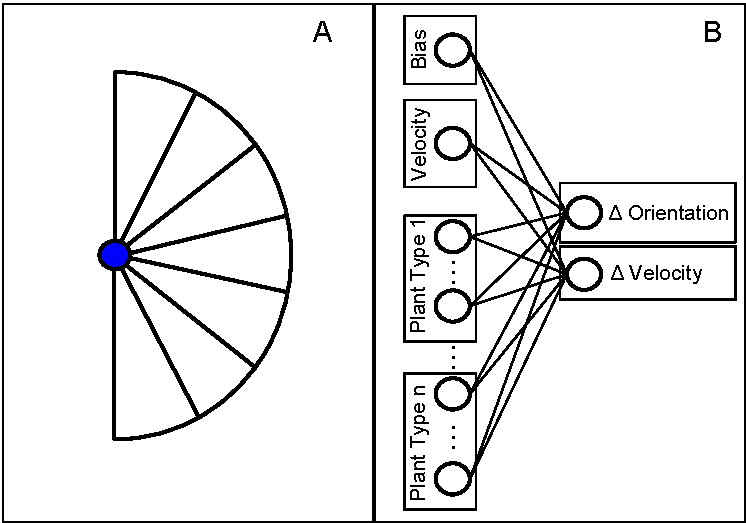
\includegraphics[scale=.65]{foraging_agent_architecture.pdf}
  \caption{The architecture of our foraging agents. A) Each agent has a $180^{\circ}$ field of vision, discretized into eight sensors for each plant type. B) Each agent is controlled by a neural network taking the agent's current velocity and sensor activations as inputs and outputting the desired change in orientation and velocity.}
  \label{fig:agent-architecture}
\end{figure}

Another important area for social learning is dynamic domains. In multiagent systems, changing conditions can negatively impact all agents if they cannot learn from one another's experience - but if they can, one agent's experience of a novel stimulus can alert other agents so they can adjust their behavior. If a social learning system is on-line, sharing updates and information about reward at every timestep, adaptation can occur rapidly.

\begin{figure}
  \centering
    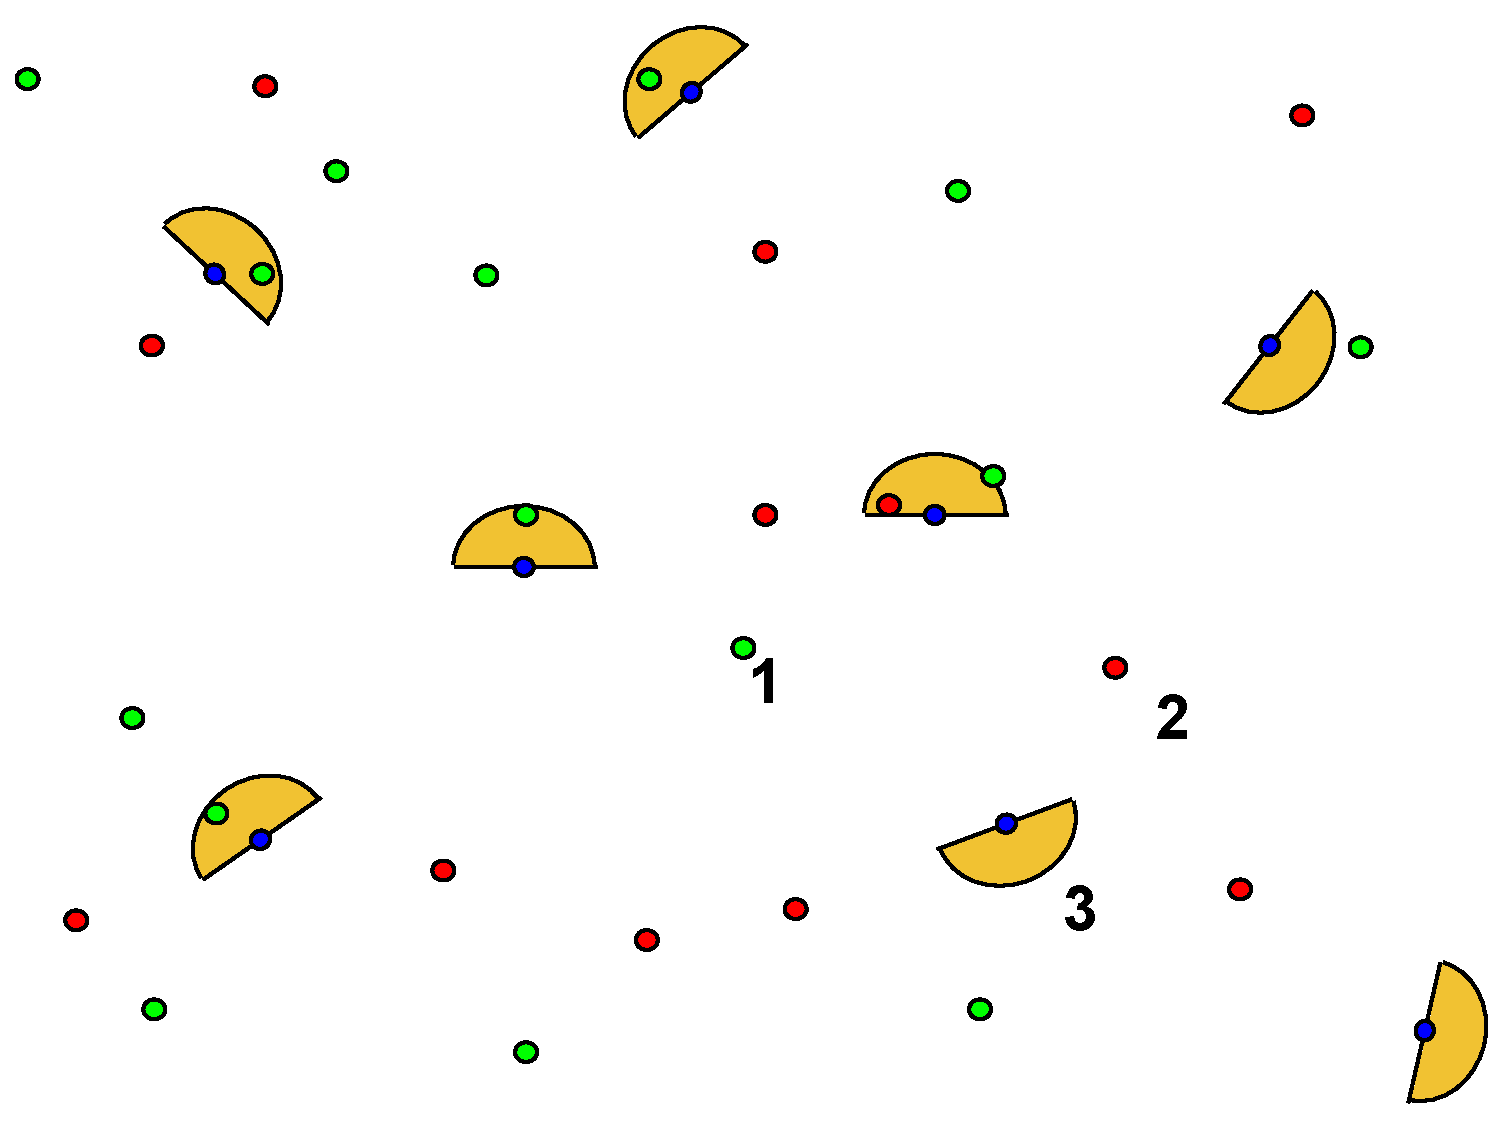
\includegraphics[scale=.3]{world.pdf}
  \caption{Our domain: a foraging world in which agents gain fitness by consuming plants which they approach.  \textbf{1} is a piece of nutritious food which increases fitness, \textbf{2} is poison which decreases fitness, and \textbf{3} is one of our agents.}
  \label{fig:foraging-world}
\end{figure}

\subsection*{Evolutionary Framework}
In this section, we discuss the framework on which we base our social learning and our modifications and extensions to this framework.

NeuroEvolution of Augmented Topologies (NEAT)\cite{stanley2002evolving} is an evolutionary algorithm that generates recurrent neural networks. Through a process of adding and removing nodes and changing weights, NEAT evolves genomes that unfold into networks. In every generation, those networks with the highest fitness reproduce, and those that have low fitness are less likely to do so. NEAT maintains genetic diversity through speciation and encourages innovation through explicit fitness sharing.

In our domain, NEAT is used to generate a population of individual neural networks that control agents in the world. The input to each network is the agent's sensors, and the outputs control the agent's velocity and orientation. The fitness of each network is determined by the success of the agent it controls - over the course of a generation, networks controlling agents who eat a good deal of rewarding food and very little poison will have high fitnesses and those which control agents with less wise dietary habits will have low fitness.

In standard NEAT, the networks that are created do not change within one generation, but in reward-based social learning, we do backpropagation\cite{rumelhart1986learning} on the networks that NEAT creates. (Because these networks are recurrent, we use backpropagation through time to do our social learning \cite{werbos1990backpropagation}.) The final fitness of each phenome, then, reflects the performance of the individual that used that phenome and elaborated on it over the course of a generation. In Darwinian evolution, the changes that were made to the phenome over the course of a generation are not saved; in Lamarkian, the genome itself is modified.

\subsection*{Prior Work}

Enhancing EAs with social and cultural learning is a flourishing area of research with a long and successful track record. We next highlight relevant prior work and explain how our approach differs from previous efforts.

Cultural algorithms \cite{reynolds1994introduction} have been used frequently in Particle Swarm Optimization (PSO) \cite{kennedy1995particle}. These algorithms maintain a ``belief space'' representing different categories of knowledge that the population has learned. New individuals are trained using this belief space in a student-teacher paradigm. In contrast, our agents maintain no separate repository of formal knowledge, but rather they learn from observations of others during their lifetime.

The ability of social learning to improve agents in a foraging domain has been explored by several researchers in recent years. Denaro et. al. \cite{denaro1996cultural} used a student-teacher model of cultural evolution without genetic inheritance and demonstrated that the population will continue to improve if Gaussian noise is added to the training examples. The NEW TIES system \cite{haasdijk2008social, vogt2010modeling} simulates a steady state evolution of decision tree agents where at each step the teacher agents probabilistically transmit their decisions and students probabilistically incorporate this knowledge. Acerbi et. al. \cite{acerbi2007social} use social learning to train embodied agents to mimic the behaviors of more experienced agents. Finally, de Oca et. al. \cite{de2011incremental} propose a methodology for incremental social learning in PSO to update Q-learning \cite{watkins1992q} value functions by randomly selecting two individuals from the population and combining their values for a given update. While all of these works are closely related and motivated by similar biological processes as our approach, they fundamentally all rely on the concept of students and teachers, and perform either no filtering or a reward-agnostic filtering of state-action pairs to be used in updating the population.


\section{Reward-Based Social Learning}
\label{sec:rbsl}

Our approach, detailed in Figure \ref{fig:flowchart} is an on-line learning algorithm that operates continuously as an agent moves in the world. At every timestep, each agent perceives the state of the world around it, and activates an internal neural network according to that state. The output of this network represents the agent's motor commands. Both the input and the output of the network are saved and stored in memory. Upon moving, an agent encountering a positive reward will retrieve its recent inputs and associated outputs from memory and train other individuals on these input-output pairs using backpropagation.

\begin{algorithm}
\begin{algorithmic}
\REQUIRE $n \geq 0 \vee x \neq 0$
\ENSURE $y = x^n$
\STATE $y \Leftarrow 1$
\IF{$n < 0$}
\STATE $X \Leftarrow 1 / x$
\STATE $N \Leftarrow -n$
\ELSE
\STATE $X \Leftarrow x$
\STATE $N \Leftarrow n$
\ENDIF
\WHILE{$N \neq 0$}
\IF{$N$ is even}
\STATE $X \Leftarrow X \times X$
\STATE $N \Leftarrow N / 2$
\ELSE[$N$ is odd]
\STATE $y \Leftarrow y \times X$
\STATE $N \Leftarrow N - 1$
\ENDIF
\ENDWHILE
\end{algorithmic}
\caption{The pseudo-code for our rewards-based social learning algorithm.}
\label{alg:rewardsbased}
\end{algorithm}

\begin{figure}
  \centering
    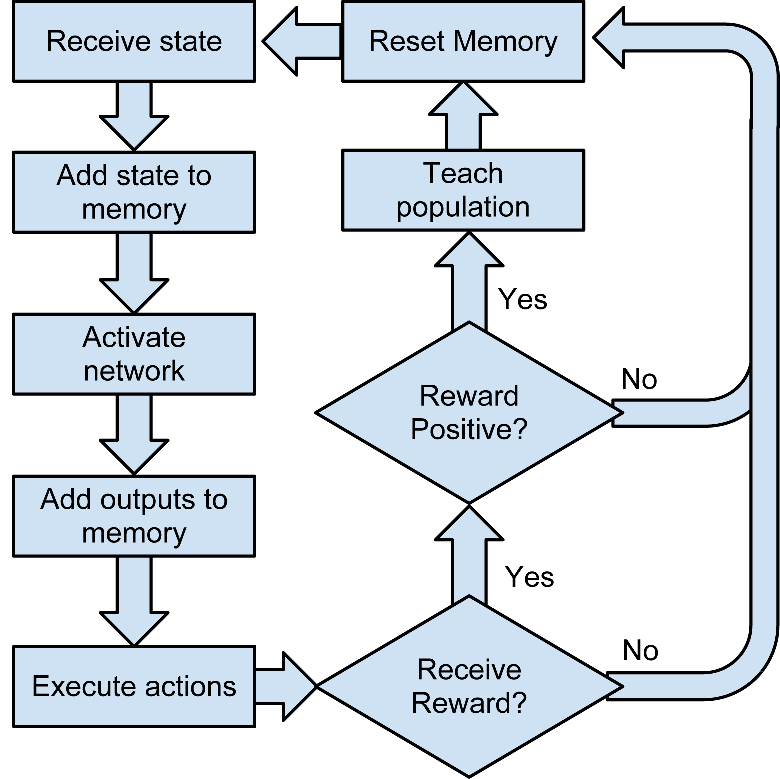
\includegraphics[scale=.6]{flowchart.pdf}
  \caption{Individuals remember their most recent inputs and the associated actions taken, and when rewarded will train other individuals on their recent actions.}
  \label{fig:flowchart}
\end{figure}


As a result of using only positive rewards to identify those actions on which we want to train agents, social learning can begin immediately in the first generation of the evolutionary algorithm. In contrast, previous approaches \cite{denaro1996cultural} instead chose strong individuals as teachers to train weaker individuals in appropriate behavior, thereby requiring at least one generation in which to identify strong individuals. Additionally, by allowing any individual to train any other, we leverage a diversity of different behaviors in problem solving.
 
\section{Experimental Setup}
\label{sec:setup}
In this section we first describe the domain in which we test our model, the inputs and outputs that our agents receive, and the common parameters across all our experiments.

\subsection*{The Foraging Domain}
    Our domain is a foraging world in which agents move freely on a continuous toroidal surface. We populate our world with various plants, some of which are considered nutritious and bear positive reward, while others are poisonous and bear negative reward. These plants are randomly distributed over the surface of the world. This foraging domain is non-competitive and non-cooperative - each agent acts independently of all other agents, with the exception of the training signals which pass between them. At the start of each generation, all individuals begin at the center of the world, oriented in the same direction, and confronted with the same plants. Every agent then has some time steps to move about the surface of the world eating plants - which happens automatically when an individual draws close - before the generation is over and a new population is evolved.
    
\subsection*{Sensors and Outputs}

  Agents ``see'' plants within a certain horizon via a collection of sensors - they have eight sensors for each type of plant, each of which detects plants in a different 12.5 degree sector of the 180 degrees ahead of the agent. Agents cannot see other individuals, or plants they have already eaten- all they can see is edible food. The strength of the signal generated by each plant is proportional to its proximity to the agent. Agents also have a sensor by which they can detect their current velocity. These sensors constitute the inputs to the neural network, and thusly the individual's state.


\subsection*{Common Parameters}

In our simple world, the toroidal surface is 2000 by 2000 units, with 50 randomly distributed plants of value 100. Our complex world has a surface of 500 by 500 units, with 20 randomly distributed plants of each value -100, -50, 0, 50, and 100. We create 100 different agents in each generation,  and divide them into 10 cultural cliques. In both worlds, there are 100 agents and when they are divided into cultural cliques, there are ten cliques of ten agents. Each agent had 8 different sensors for each type of plant, and automatically ate any plant it came within 5 units of. Each generation lasted 1000 timesteps, and each experiment was averaged over 30 runs.

\section{Results}
\label{sec:results}
In this section we review the results of our experimentation.  We have four experiments, viz. Reward-Based Learning with and without Evolution, Darwinian and Lamarkian Evolution, Population-Wide and Cultural Evolution, and Reward-Based Learning and Student-Teacher Learning.   The first three experiments each examine a different part of our final algorithm for reward-based learning and the motivation and experimental results for each of them.  The last compares our algorithm with a recent student-teacher learning algorithm, and shows that our reward-based social learning produces excellent results faster.

\begin{figure}
  \centering
    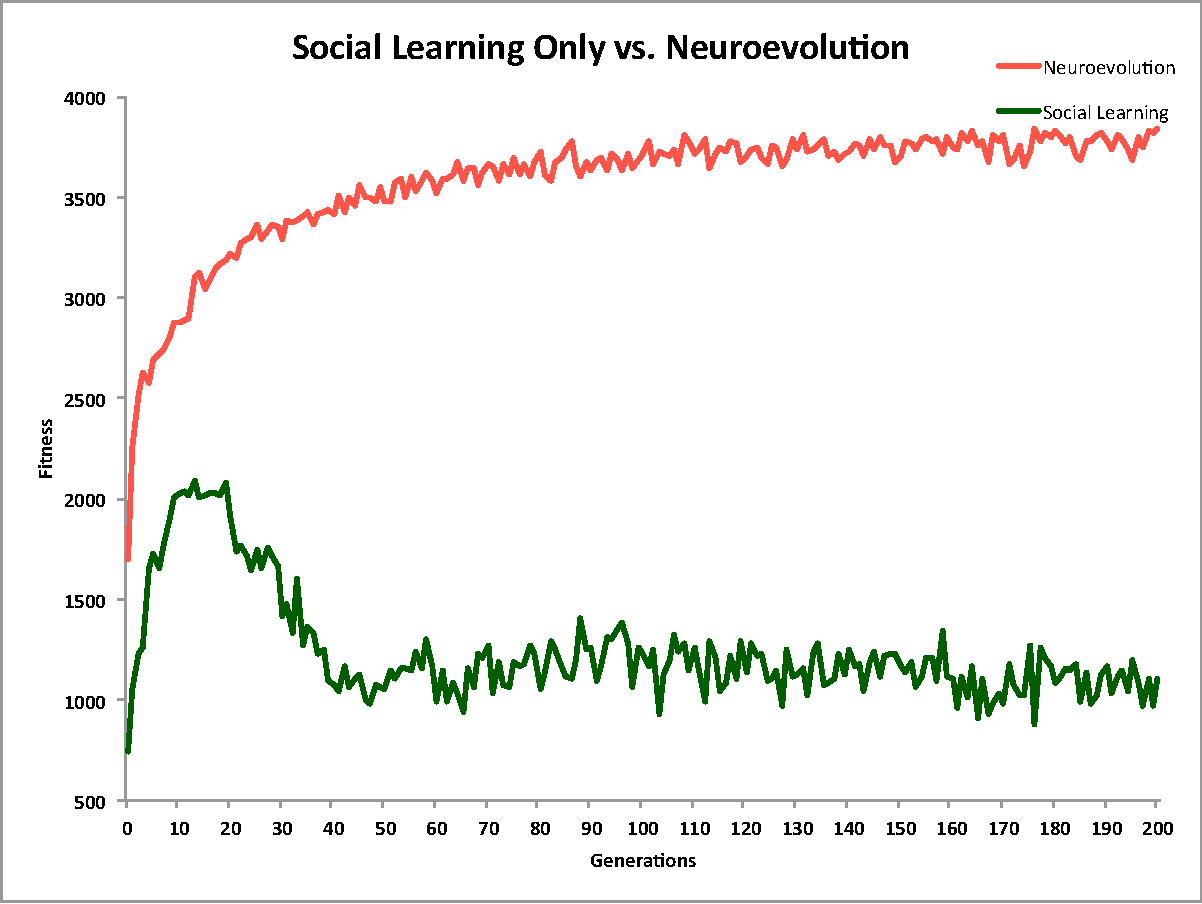
\includegraphics[scale=.35]{social_learning_vs_neuroevolution.pdf}
  \caption{Pure reward-based learning collapses after several generations, while neuroevolution alone converges to a stable but suboptimal solution.}
  \label{fig:social-neuro}
\end{figure}

\subsection*{Reward-Based learning vs. Neuroevolution}

Our first experiment was to examine the effect of pure reward-based learning without evolution to the effect of pure neuroevolution.  As our results in Figure \ref{fig:social-neuro} show, while reward-based learning alone is effective initially at improving, after several epochs a regression to the mean approach is observed in which the entire population converges to a mediocre average score. A similar effect has been observed in previous social learning experiments \cite{denaro1996cultural}.   Neuroevolution, our baseline algorithm, is significantly better at discovering strong solutions. 


\subsection*{Darwinian vs. Lamarkian evolution}

Genetic inheritance paradigms in evolution fall into one of two main categories: Darwinian and Lamarkian. In Darwinian evolution, individual genomes are fixed and any knowledge or abilities gained during their lifetimes are not passed on to their offspring at birth. By contrast, in Lamarkian evolution an individual's genome changes as it learns throughout its life, and these changes are passed on to each of its offspring. In the context of our experiments, this corresponds to whether the changes in each individual's neural network weights are propagated to their genome at the end of the generation.

\begin{figure}
  \centering
    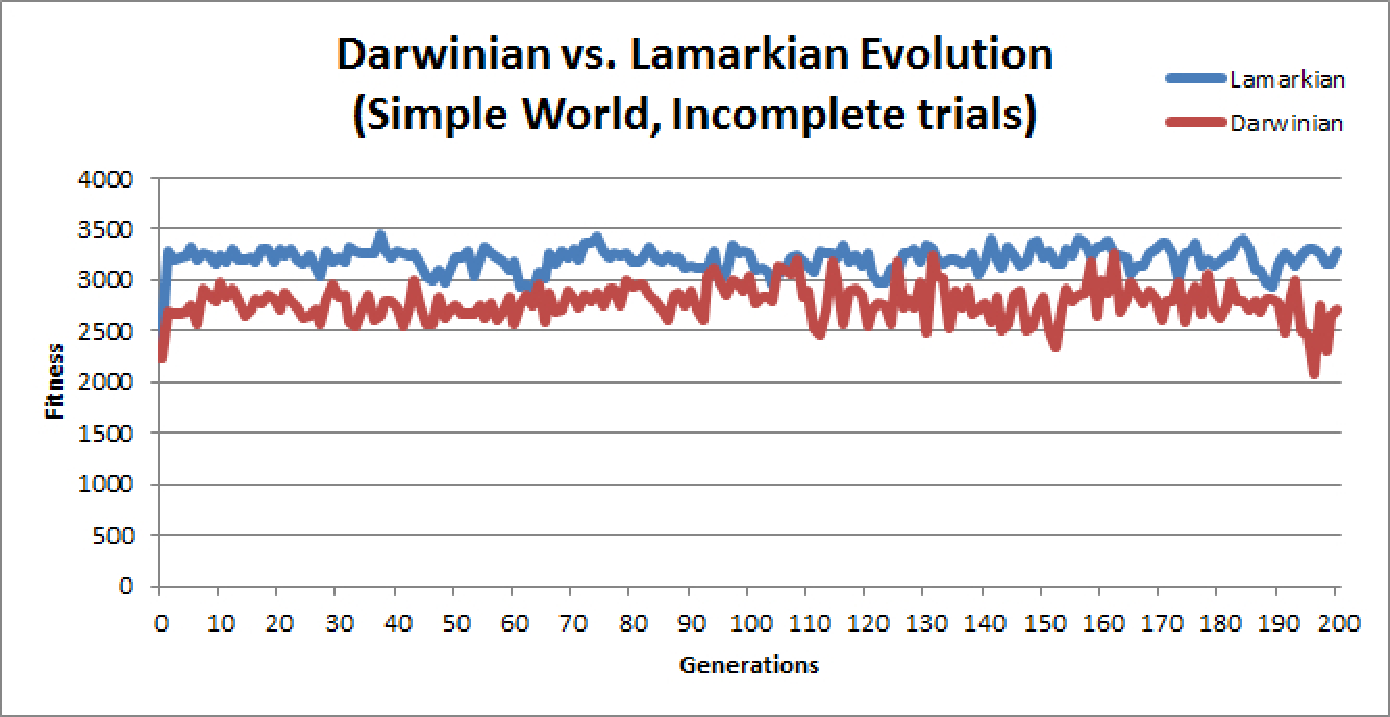
\includegraphics[scale=.35]{darwinian_vs_lamarkian_evolution.pdf}
  \caption{Lamarkian learning is more effective than Darwinian and converges more rapidly.}
  \label{fig:darwin-lamark}
\end{figure}


Figure \ref{fig:darwin-lamark} shows the results of applying our non-hierarchical social learning algorithm to the foraging domain for both the Lamarkian and Darwinian paradigms. These results indicate that Lamarkian evolution is able to quickly reach a near-optimal score but then proceeds to degrade slowly over time. In  \textit{on-line} evolutionary learning algorithms, it has been shown \cite{whiteson2006evolutionary} that Darwinian evolution is preferable to Lamarkian evolution in dynamic environments where adaptation is essential and the Baldwin effect \cite{simpson1953baldwin} may be advantageous. As adaptation is not necessary for our agents (i.e., the rewards of each plant type are the same in every generation), it is not exceedingly surprising that Lamarkian evolution initially outperforms Darwinian evolution.


\subsection*{Population vs. Cultural Learning}
While Lamarkian social learning is able to find good results quickly, it takes an extremely long time and is likely to provide redundant information.  Moreover, harmfully mutated agents will train all other agents in the population on bad behavior.  In order to address this problem, we form 10 cliques in the population of 10 agents each, and have agents within each of these cliques only learn from one another.  This cultural variant of reward-based learning increases behavioral diversity relative to learning from the entire population (Figure \ref{fig:orientation} and Figure \ref{fig:velocity}) , and   decreases the number of iteration of backprop by a factor of ten.

\begin{figure}
  \centering
    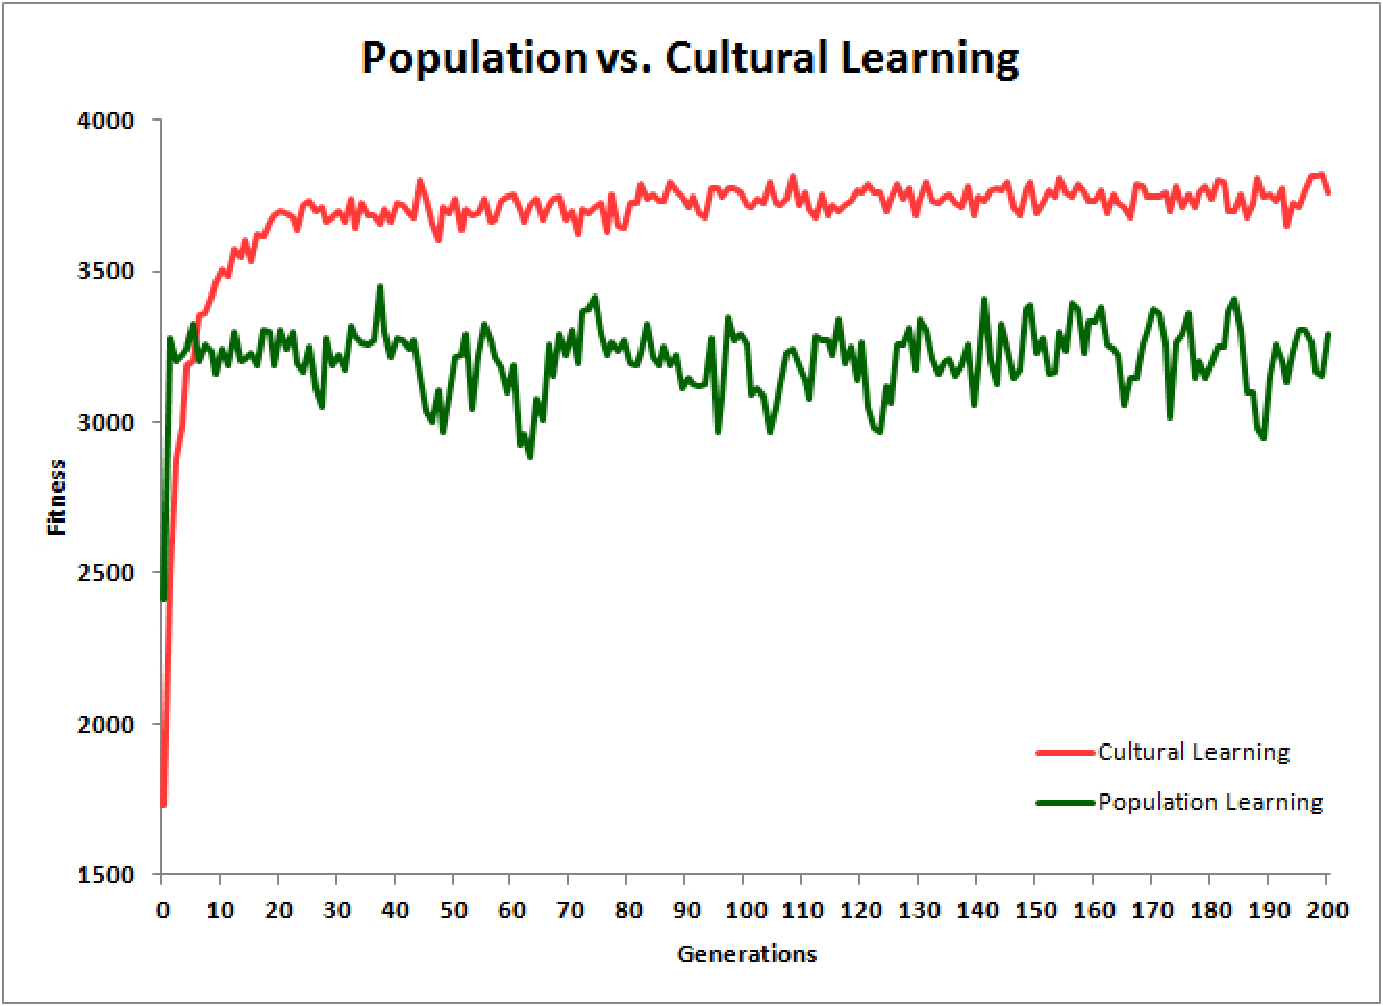
\includegraphics[scale=.35]{population_vs_cultural_learning.pdf}
  \caption{The results of agents learning from observations of the entire population compared to only agents in the same clique.}
  \label{fig:population-social}
\end{figure}ls

Figure \ref{fig:population-social} shows the results comparing population-based and cultural social learning. Interestingly, the cultural social learning not only reaches a higher peak than the population based method, but also arrives at this level of fitness more rapidly.  Preventing agents who have behavior that is harmful from impacting the remainder of the population provides safety and protection; when every mutated organism has the opportunity to train every other, as is the case in population-wide learning, the entire population may be negatively impacted.  Because cultural evolution is more efficient and provides better results, likely due to this protection from mutation and the fostering of diversity, we use it in our final model.

\begin{figure}
  \centering
    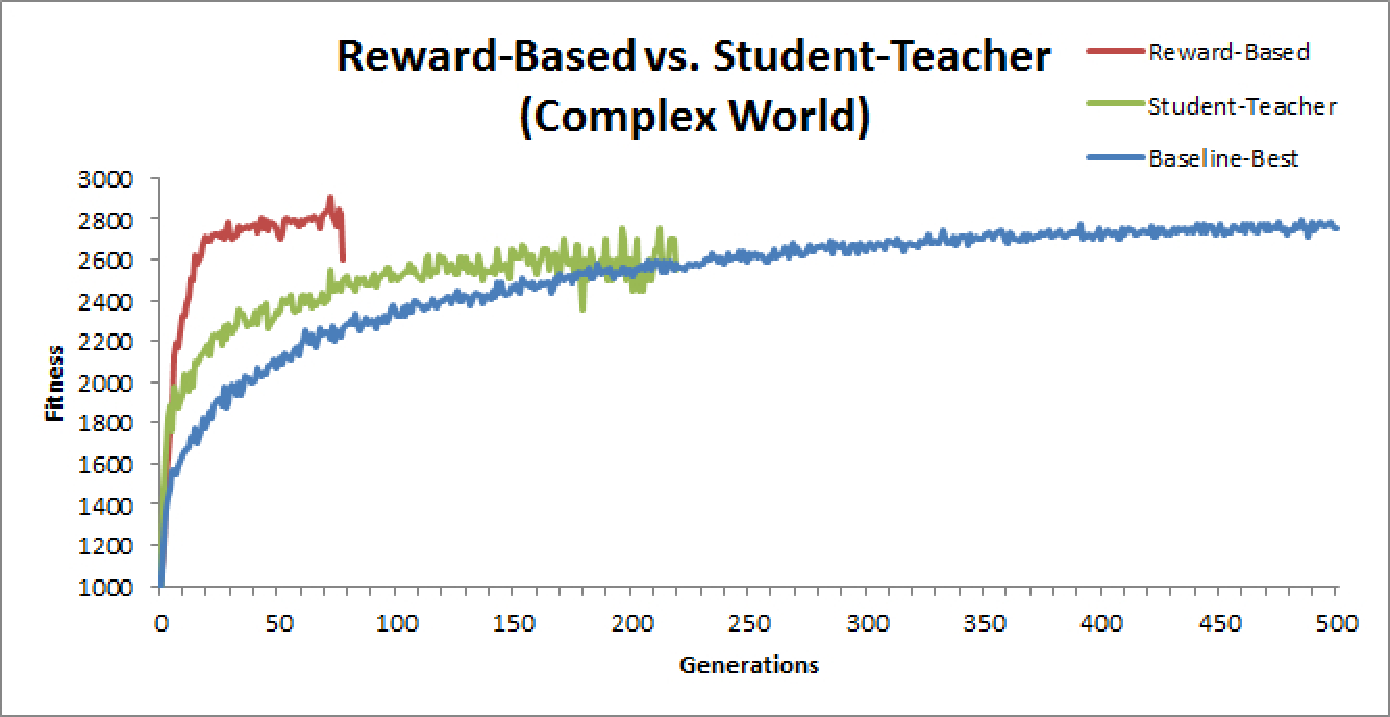
\includegraphics[scale=.35]{reward_based_vs_student_teacher.pdf}
  \caption{The results of our algorithm in a complex world evaluated alongside a more traditional student-teacher model and baseline pure neuroevolution.}
  \label{fig:reward-studetteacher}
\end{figure}

\subsection*{Reward-Based Learning vs. Student-Teacher Learning}
Finally, we compare our evolutionary, Lamarkian, cultural reward-based algorithm to a version of student-teacher learning based on the NEW TIES system \cite{haasdijk2008social} which chooses champions of previous generations to be teachers, and at every timestep probabilistically teaches the lowest-fitness member of each clique the response of the generation of the previous generation.  This student-teacher model works and outperforms baseline, but our model, which filters on each training example by reward rather than by filtering on individuals outperforms it.

Figure REFFIGURE shows our results.  Reward-based learning converges to a near-optimal solution very rapidly in both the simple and the complex world.  In the simple world, student-teacher learning eventually reaches a slightly superior solution, after much more computational effort.  In the complex world, not only does social learning reach a better solution than student-teacher learning, it also converges to that solution several orders of magnitude faster.  

\section{Discussion and Future Work}
\label{sec:future}


In this section we discuss possible mechanisms at work in and areas for exploration in the domain of reward-based social learning.  We then discuss potential future work that could be done to exploit these phenomena and improve reward-based social learning as both a model of artificial life and a machine learning algorithm. 


\begin{figure}
  \centering
    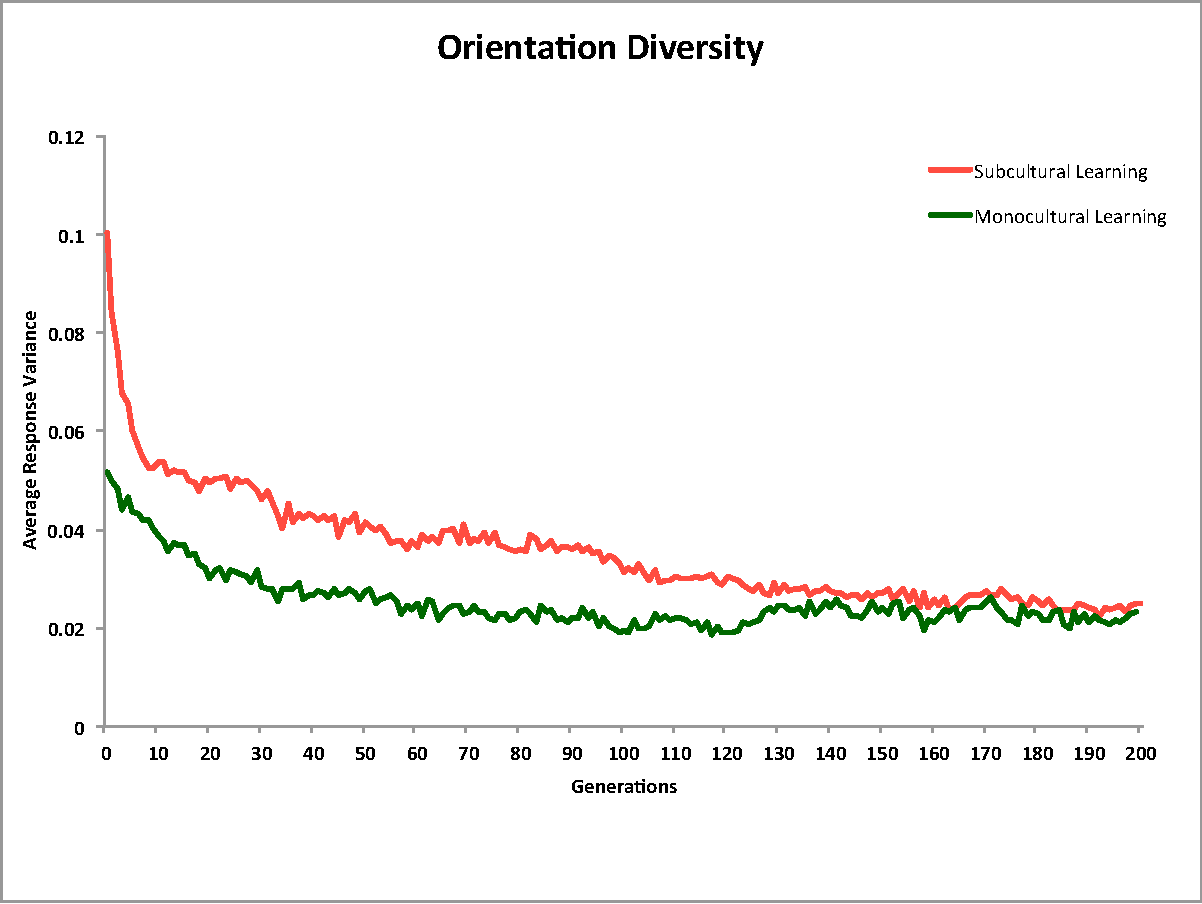
\includegraphics[scale=.35]{orientation_diversity.pdf}
  \caption{In the cultural learning model, diversity in terms of orientation is maintained for longer than in population learning before behavior converges.}
  \label{fig:orientation}
\end{figure}

\begin{figure}
  \centering
    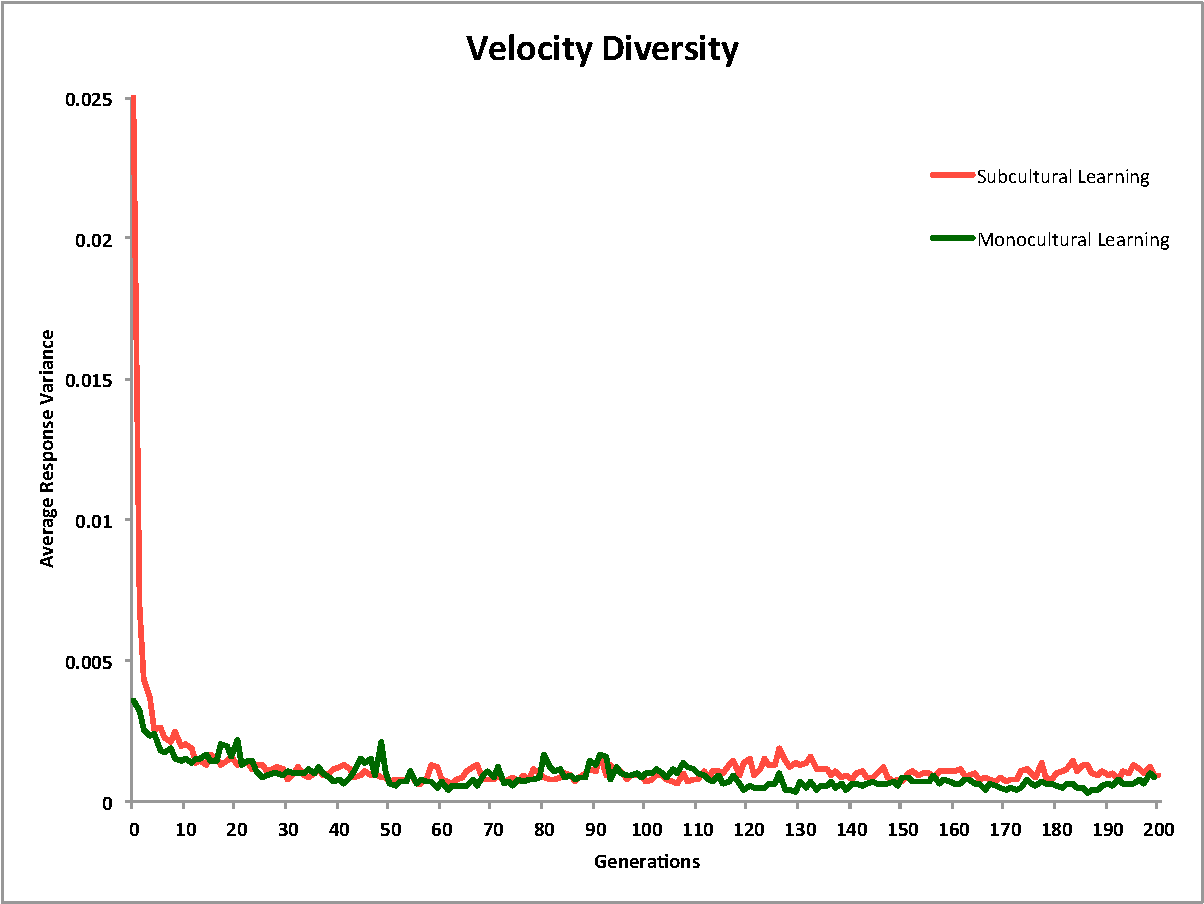
\includegraphics[scale=.35]{velocity_diversity.pdf}
  \caption{Velocity converges more quickly in the cultural model than in the population model.}
  \label{fig:velocity}
\end{figure}


By preserving the diversity of behavior present in the entire population and presenting all agents with information from other agents in the same environment, our algorithm leverages the advantages of both evolution and cultural learning. Interestingly, by dividing our population into cultural groups of ten agents, we were able to maintain a higher level of performance than via individuals not communicating, or communicating with a larger population.  By both maintaining diversity (a task which is anathema to student-teacher learning and difficult in full population learning) and keeping agents from being negatively impacted by harmful agents making and teaching bad decisions, our cultural reward-based algorithm works better than any other.

Future work may involve investigating the relationship between this and other forms of social learning and Q-learning.  Additionally, one strength of non-hierarchical social learning is its ability to transmit information about novel situations to all agents without those agents having to experience those situations themselves.  As such, investigating the impact of non-hierarchical social learning in dynamic domains with changing rewards is a promising and practical avenue for new research.  Finally, our current model teaches agents about the previous timestep with one iteration of backprop whenever there is a reward.  Extending the model to account for the magnitude of the reward, and to store and train on information about previous timesteps may lead to new insights.   

\section{Conclusions}
\label{sec:conclusions}

We have presented a reward-based approach to apply social learning in evolutionary algorithms that converges to better solutions faster than previous known solutions. Traditionally, social learning in evolutionary algorithms has followed a student-teacher model that assigns roles to each agent. Our approach removes this hierarchy and instead updates individuals based on actions taken by \textit{any} agent that lead to a positive reward.  Further filtering of results by constraining teaching samples to those from the same cultural group results in further improvement to performance.  Experiments in a complex robot foraging domain demonstrate that this approach is highly effective at quickly learning a near-optimal policy with Lamarkian evolution. 

\bibliographystyle{abbrv}
\bibliography{sigproc}
\end{document}